\nonstopmode
\documentclass{article}

\usepackage[utf8]{inputenc}
\usepackage{geometry}
\usepackage{graphicx}
\usepackage{polski}
\usepackage{subcaption}
\setlength{\parindent}{0pt}

\graphicspath{ {images/} }
\geometry{legalpaper, portrait, margin=1in}

\title{\LARGE Algorytmy z powracaniem\\ Sprawozdanie nr 4}
\author{Adam Piaseczny \\	151757 \and
				Igor Szczepaniak \\ 151918}
\date{Grupa piątkowa 11:45}

\begin{document}

\maketitle
\pagebreak

\tableofcontents
\pagebreak

\section{Wprowadzenie}

W tym sprawozdaniu zbadaliśmy znaczenie gęstości i ilości wierzchołków przy wyszukiwaniu cykli Hamiltona oraz cyklu Eulera w grafach nieskierowanych. Kod źródłowy został napisany w języku \textbf{python} ze względu na prostotę implementacji. Wygenerowaliśmy 15 losowych grafów nieskierowanych $G=(V,E)$ o rożnych $|V|=n$ posiadających cykl Hamiltona oraz Eulera.

\section{Wstęp teoretyczny}

Droga Eulera to ścieżka w grafie, która przechodzi przez każdą jego krawędź dokładnie raz. Jeśli droga Eulera zaczyna się i kończy na tym samym wierzchołku, stanowi cykl Eulera. Warunkiem koniecznym i dostatecznym istnienia cyklu Eulera jest parzystość stopnia wszystkich wierzchołków oraz spójność grafu. Dla każdego grafu zmierzyliśmy ilość czasu potrzebną na znalezienie cyklu Eulera dla danego $n$, czas ten będzie oznaczony jako $t_E$.  Sprawdzanie istnienia cyklu Eulera w grafie może być osiągnięte następującym algorytmem:

\begin{itemize}
	\item algorytm drogaEulera($V$):
	\item Iterujemy przez wszystkie krawędzie $E$ wychodzące z wierzchołka $V$
	\begin{enumerate}
		\item Usuwamy krawędź $E$ z grafu i zapisujemy sąsiadujący wierzchołek $U$
		\item Uruchamiamy drogaEulera dla $U$
	\end{enumerate}
	\item Dodajemy V do rozwiązania
\end{itemize}

Algorytm ten ma złożoność $O(m)$ i zależy od liczby krawędzi $m=\frac{d}{2}\times n \times (n-1)$, gdzie $d$ jest gęstością grafu. Złożoność wynika z faktu odwiedzenia każdej krawędzi w grafie dokładnie raz oraz usuwania odwiedzonej krawędzi w stałym czasie. Dodatkowo do całkowitego czasu wykonania algorytmu wlicza się również czas wyszukania kolejnej krawędzi $E$ wychodzącej z wierzchołka $V$, czas ten jest zależny od reprezentacji grafu co wyjaśniliśmy w dalszej części pracy.

Cykl Hamiltona to taki cykl w grafie, w którym każdy wierzchołek grafu odwiedzany jest dokładnie raz (oprócz pierwszego wierzchołka). Sprawdzenie czy graf posiada cykl Hamiltona opiera się na generowaniu permutacji kolejnych możliwych ścieżek z danego wierzchołka do nieodwiedzonych wierzchołków sąsiadujących. Posiadając wszystkie możliwe ścieżki możemy zweryfikować czy są one cyklami Hamiltona.

\section{Prezentacja wyników}

Czasy wyszukiwania pierwszego cyklu Eulera i Hamiltona w grafie oznaczyliśmy jako $t_E$ i $t_{H1}$, a wyszukiwanie wszysktich cykli Hamiltona oznaczyliśmy jako $t_{HA}$. Poniższa tabela przedstawia wyniki dla gęstości grafu równej $d=0.6$.

\begin{figure}[h!]
\centering
  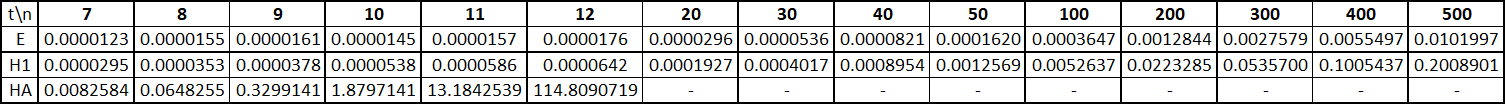
\includegraphics[width=1.0\linewidth]{zad2_tabela.png}
	\captionof{figure}{Prezentacja wyników - tabela}
\end{figure}%

Z wyników z stworzyliśmy następujący wykres:

\begin{figure}[h!]
\centering
  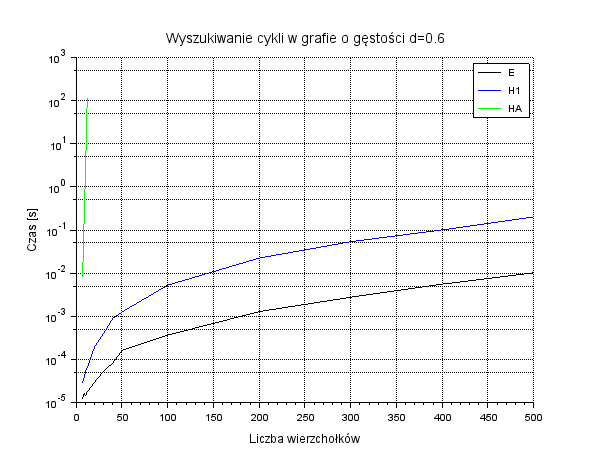
\includegraphics[width=0.5\linewidth]{zad2_wykres.png}
	\captionof{figure}{Prezentacja wyników}
\end{figure}%

Czas wykonywania algorytmu znajdywania cyklu Eulera jest niższy niż czas wyszukiwania pierwszego cyklu Hamiltona, wynika to z różnic złożoności powyższych algortymów. Znajdywanie cyklu Eulera należy do problemów klasy P - jest to problem decyzyjny, gdzie rozwiązanie można znaleźć w czasie wielomianowym. Algorytm znajdywania cyklu Eulera opiera się na algorytmie DFS, który w takim czasie przebiega. Do złożoności $O(m)$ algorytmu znajdywania cyklu Eulera należy dodać czas wyszukania kolejnej krawędzi. Lista sąsiadów jest odpowiednia dla tego zadania, gdyż może zwrócić kolejną krawędź w czasie $O(1)$ (przy usuwaniu odwiedzonych krawędzi w stałym czasie).

Znajdywanie cyklu Hamiltona jest problemem klasy silnie NP-zupełnych, co znaczy, że nie istnieje algorytm rozwiązujący ten problem w czasie wielomianowym; rozwiązanie problemu jest jednoznaczne ze znalezieniem takiego cyklu, lub wykazaniem jego braku. Liczba możliwych ścieżek w grafie wynosi $n!$, więc algorytm sprawdzający istnienie cykli Hamiltona ma złożoność $O(n!)$. Wraz ze wzrostem liczby wierzchołków $n$ czas wykonywania algorytmu drastycznie się zwiększa, przez co przebieg algorytmu dla większych wartości $n$ może okazać się nieopłacalny ze względu na czas wykonywania - z tego powodu przy wyszukiwaniu wszystkich cykli Hamiltona w grafie nie wykonywaliśmy testów dla wartości $n$ większej niż 12 ponieważ już dla 13 wierzchołków uznaliśmy czas działania algorytmu za zbyt długi. Złożoność algorytmu zarówno przy znajdywaniu pierwszego cyklu Hamiltona, jak i wszystkich istniejących w danym grafie jest taka sama, ponieważ w najgorszym przypadku przy poszukiwaniu pierwszego cyklu Hamiltona wygerenujemy $(n-1)!$ kandydatów na rozwiązanie.

\section{Cykle Eulera}

Każdy generowany przez nas graf posiadał cykl Eulera. Upewniliśmy się, że generowany graf jest Eulererowski w następujący sposób:

\begin{enumerate}
	\item Generujemy losowy graf
	\item Upewniamy się, czy graf jest spójny za pomocą jednego przebiegu algorytmu DFS, jeśli nie - generujemy go ponownie
	\item Tworzymy listę wierzchołków z nieparzystymi stopniami
	\begin{enumerate}
		\item Jeśli długość listy jest nieparzysta, powtarzamy generację grafu
		\item Łączymy krawędziami dwa losowo wybrane wierzchołki z tej grupy do momentu wyczerpania listy
	\end{enumerate}
\end{enumerate}

Kończąc ten algorytm posiadamy graf spójny posiadający parzysty stopień przy każdym wierzchołku, co jest warunkiem koniecznym i dostatecznym istnienia cyklu Eulera w grafie. Sprawdziliśmy czas wykonywania algorytmu wyszukiwania cyklu Eulera i oznaczyliśmy go jako $t_E$ dla gęstości $d=0.2$ oraz $d=0.6$. Wyniki przedstawiliśmy w następującej tabeli:

\begin{figure}[h!]
\centering
  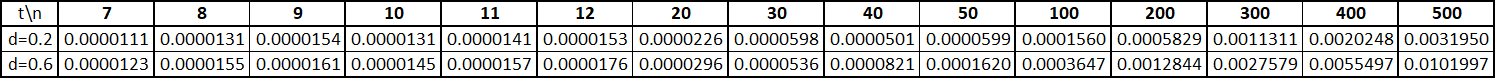
\includegraphics[width=1.0\linewidth]{zad3_tabela.png}
	\captionof{figure}{Cykle Eulera - tabela}
\end{figure}%

Z wyników z stworzyliśmy następujący wykres:

\begin{figure}[h!]
\centering
  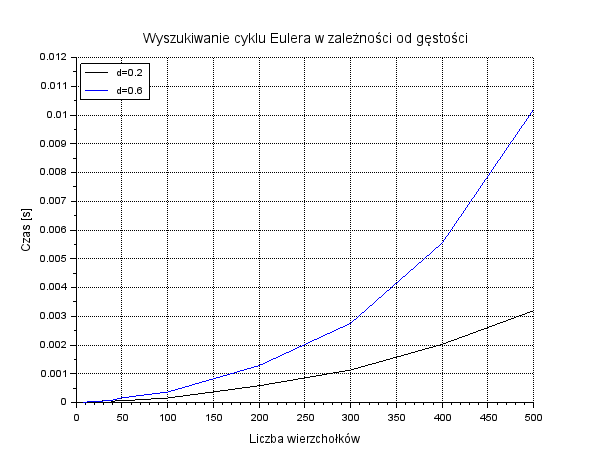
\includegraphics[width=0.5\linewidth]{zad3_wykres.png}
	\captionof{figure}{Cykle Eulera}
\end{figure}%

Na wykresie zauważyliśmy zależność między gęstością grafu a długością czasu wyszukiwania cyklu Eulera w grafie, dzieje się tak ponieważ algorytm jest wrażliwy na liczbę krawędzi w grafie. Czas wykonywania algorytmu wraz ze wzrostem liczby wierzchołków rośnie ponieważ dla tej samej gęstości liczba krawędzi $m$ jest zależna od liczby wierzchołków $n$.

\pagebreak

\section{Cykle Hamiltona}

Algorytm z powracaniem to ogólny algorytm wyszukiwania wszystkich rozwiązań problemów obliczeniowych, który stopniowo generuje kandydatów na rozwiązanie, jednak gdy stwierdzi, że dany kandydat nie może być poprawnym rozwiązaniem, nawraca do punktu, gdzie może podjąć inną decyzję. Przykładem takiego algorytmu jest nasza implementacja wyszukiwania cykli Hamiltona w grafie przy reprezentacji listy sąsiadów, którą wybraliśmy ze względu na szybkość otrzymywania zbioru sąsiadów (od $O(1)$ do $O(n)$). Algorytmy z powracaniem mogą być zastosowane do wielu innych problemów, które wymagają stopniowego generowania częściowych odpowiedzi - przykładowym problemem może być automatyczne rozwiązywanie krzyżówek, gdzie kandydatów na odpowiedź do danego hasła może być wielu, a o poprawności dowiadujemy się dopiero przy późniejszej analizie pozostałych haseł. Zmierzyliśmy czas wyszukiwania pierwszego cyklu Hamiltona $t_{H1}$. W poniższej tabeli przedstawiliśmy wyniki dla poszukiwania pierwszego cyklu Hamiltona w grafie dla gęstości $d=0.2$ oraz $d=0.6$.

\begin{figure}[h!]
\centering
  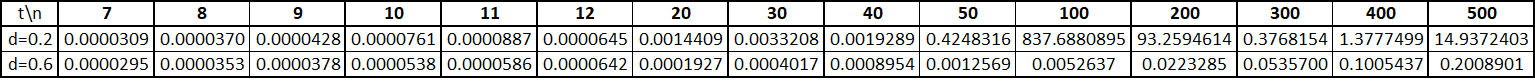
\includegraphics[width=1.0\linewidth]{zad4_H1_tabela.png}
	\captionof{figure}{Cykle Hamiltona - tabela}
\end{figure}%

Z wyników z stworzyliśmy następujący wykres:

\begin{figure}[h!]
\centering
  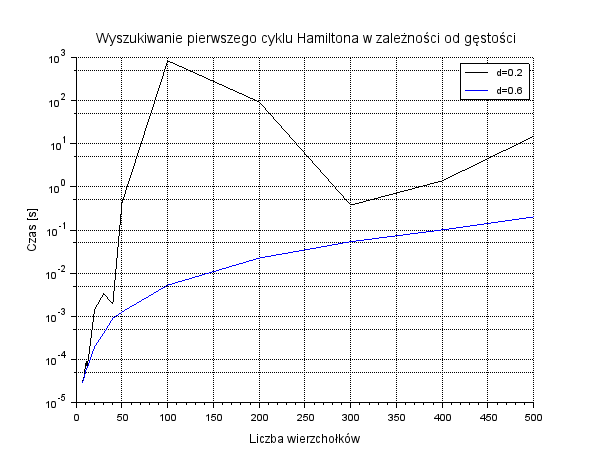
\includegraphics[width=0.5\linewidth]{zad4_H1_wykres.png}
	\captionof{figure}{Cykle Hamiltona}
\end{figure}%

Zmierzyliśmy również czas wyszukiwania wszystkich istniejących cykli Hamiltona w grafie $t_{HA}$. Wyniki przedstawiliśmy w poniższej tabeli dla gęstości $d=0.2$ oraz $d=0.6$ :

\begin{figure}[h!]
\centering
  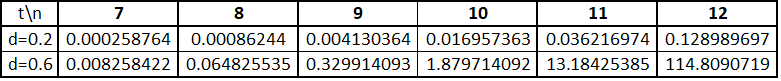
\includegraphics[width=0.7\linewidth]{zad4_HA_tabela.png}
	\captionof{figure}{Wszystkie cykle Hamiltona - tabela}
\end{figure}%

Z wyników z stworzyliśmy następujący wykres:

\begin{figure}[h!]
\centering
  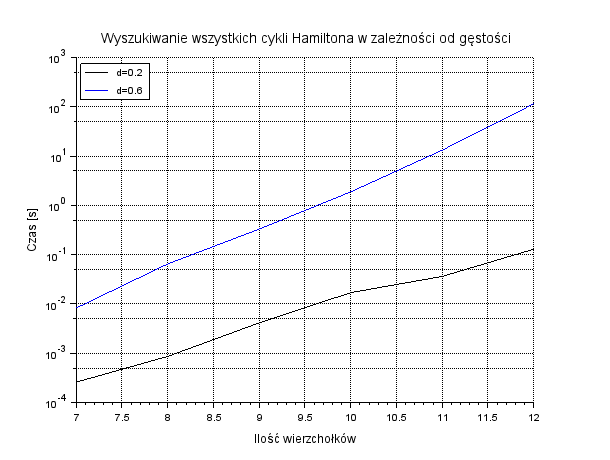
\includegraphics[width=0.5\linewidth]{zad4_HA_wykres.png}
	\captionof{figure}{Wszystkie cykle Hamiltona}
\end{figure}%

Zarówno dla wyszukiwania pierwszego cyklu Hamiltona jak i wszystkich cykli Hamiltona w grafie wykorzystaliśmy ten sam algorytm, z tą różnicą, że przy wyszukiwaniu pierwszego cyklu Hamiltona przerywamy algorytm po jego znalezieniu. Czas znajdywania wszystkich cykli Hamiltona jest dłuższy od znajdywania pierwszego cyklu z racji przejścia wszystkich możliwych ścieżek w grafie (których jest więcej przy większej gęstości grafu). Fakt odwiedzenia każdej ścieżki powoduje, że czas znajdywania wszystkich cykli Hamiltona jest bardziej przewidywalny niż znajdywania pierwszego cyklu.

Podczas szukania pierwszego cyklu Hamiltona istnieje szansa znalezienia rozwiązania przy pierwszym zagłębieniu rekurencyjnym ($O(n)$), ale jest też możliwość znalezienia tego rozwiązania w najgorszym przypadku po $(n-1)!$ przejściach rekurencyjnych (dla grafu pełnego). Czyni to szukanie pierwszego cyklu bardzo mało "stabilnym" pod wględem czasu wykonania. Ponadto im większa jest gęstość grafu tym czas wykonania algorytmu jest mniejszy i bardziej przewidywalny - jest większa szansa na znalezienie pierwszego cyklu Hamiltona z powodu większej liczby cykli w grafie z większą liczbą krawędzi. Sprawdziliśmy liczbę cykli Hamiltona $C_H$ i przedstawiliśmy je w poniższej tabeli dla gęstości $d=0.2$ oraz $d=0.6$.

\begin{figure}[h!]
\centering
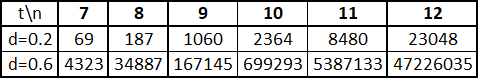
\includegraphics[width=0.6\linewidth]{zad4_CYC.png}
\captionof{figure}{Liczba cykli - tabela}
\end{figure}%

Zauważyliśmy znaczącą zależność pomiędzy liczbą cykli Hamiltona w grafie a gęstością tego grafu co tłumaczy różnicę w przewidywalności czasu wykonania algorytmu szukania pierwszego cyklu Hamiltona.

\end{document}
